\documentclass[10pt,a4paper]{article}
\usepackage[utf8]{inputenc}
\usepackage[english,spanish]{babel}
\usepackage{indentfirst}
\usepackage{anysize} % Soporte para el comando \marginsize
%\marginsize{1.5cm}{1.5cm}{0.5cm}{1cm}
\marginsize{2,5cm}{1,8cm}{4cm}{1,7cm}
\usepackage[psamsfonts]{amssymb}
\usepackage{amssymb}
\usepackage{amsfonts}
\usepackage{amsmath}
\usepackage{amsthm}
\usepackage{multicol,caption}
\usepackage{blindtext}
\usepackage{graphicx}
\newtheorem{thm}{Teorema}[section]
\newtheorem{cor}[thm]{Corolario}
\newtheorem{lem}[thm]{Lema}
\newtheorem{prop}[thm]{Proposición}
\theoremstyle{definition}
\newtheorem{defn}[thm]{Definición}
\theoremstyle{remark}
\newtheorem{rem}[thm]{Observación}
\def\RR{\mathbb{R}}
\def\ZZ{\mathbb{Z}}
\newcommand{\abs}[1]{\left\vert#1\right\vert}
\usepackage{stackrel}

%--------------------------------------------------------------------------
\DeclareMathOperator{\Jac}{Jac}
\renewcommand{\thepage}{}

\newenvironment{Figure}
  {\par\medskip\noindent\minipage{\linewidth}}
  {\endminipage\par\medskip}

\columnsep=7mm

%%%%%%%%%%%%%%%%%%%%%%%%%%%%%%%%%%%%%%%%
\newtheorem{definicion}{Definici\'on}[section]
\newtheorem{teorema}{Teorema}[section]
\newtheorem{prueba}{Prueba}[section]
\newtheorem{prueba*}{Prueba}[section]
\newtheorem{corolario}{Corolario}[section]
\newtheorem{observacion}{Observaci\'on}[section]
\newtheorem{lema}{Lema}[section]
\newtheorem{ejemplo}{Ejemplo}[section]
\newtheorem{solucion*}{Soluci\'on}[section]
\newtheorem{algoritmo}{Algoritmo}[section]
\newtheorem{proposicion}{Proposici\'on}[section]

\linespread{1.4} \sloppy

\newcommand{\R}{\mathbf{R}}
\newcommand{\N}{\mathbf{N}}
\newcommand{\C}{\mathbb{C}}
\newcommand{\Lr}{\mathcal{L}}
\newcommand{\fc}{\displaystyle\frac}
\newcommand{\ds}{\displaystyle}

\DeclareMathOperator{\Dom}{Dom}

%%%%%%%%%%%%%%%%%%%%%%%%%%%%%%%%%%%%%%%%

\renewcommand{\thefootnote}{\fnsymbol{footnote}}

\begin{document}
\begin{center}
 {\Large \textbf{CADENAS DE MARKOV}}
\end{center}
\begin{center}
Calixtro Ames Cynthia Lizeth $1$, Nesiosup Vilca Marcia Paulina $2$\\
Huamaní Inga Alex Raúl $3$, Romero Gómez Yasmyn Stephany $4$\vskip12pt
{\it E.P.Ciencia de la computación $1$, Facultad de Ciencias $1$, Universidad Nacional de Ingeniería $1$, e-mail:ccalixtroa@uni.pe \\E.P.Matemática $2$, Facultad de Ciencias $2$, Universidad Nacional de Ingeniería $2$, e-mail:marcia.nesiosup@gmail.com \\ E.P.Matemática $3$, Facultad de Ciencias $3$, Universidad Nacional de Ingeniería $3$, e-
mail:ahuamanii@uni.pe \\E.P.Matemática $4$, Facultad de Ciencias $4$,Universidad Nacional de Ingeniería$4$, e- mail:}
\end{center}
%\maketitle 
\begin{quotation}
{\small
\begin{abstract}
\noindent  Una cadena de Markov es una serie de eventos, en la cual la probabilidad de que ocurra un evento depende del evento inmediato anterior. En efecto, las cadenas de este tipo tienen memoria, $"recuerdan"$ el último evento y esto condiciona las posibilidades de los eventos futuros. Esta dependencia del evento anterior distingue a las cadenas de Markov de las series de eventos independientes, como tirar una moneda al aire o un dado. En el presente estudio implementamos la simulación de 3 diferentes tipos de cadenas de Markov (irreductibles,periódicas y estacionarias).

\end{abstract}
\hspace*{0.5cm} Palabras Claves:Cadenas, Markov, Implementación, Estocástico.  
}\\
{\small
\hspace*{0.5cm} 

Keywords: Chains, Markov, Implementation, Estochastic. \\ 
}
\end{quotation}
\begin{multicols}{2}
\begin{center}
\section{INTRODUCCIÓN}
\end{center}
Para una mejor comprensión de las cadenas de Markov y la posterior simulación de algunos ejemplos empezaremos por establecer algunos conceptos previos requeridos.
\subsection{CONCEPTOS}
\textbf{\textit{Procesos Estocásticos}}\\
Un proceso estocástico se puede definir equivalentemente de las siguientes dos maneras.\\
1. Como un conjunto de realizaciones temporales y un índice aleatorio que selecciona una 
de ellas.\\
2. Como un conjunto de variables aleatorias $X_{t}$ indexadas por un índice $t$ , dado que $t \in T$ con $T\subseteq \mathbb{R} $.\\\\
Un proceso estocástico se dice de \textbf{\textit{tiempo continuo}} si $T$ es un intervalo (usualmente este intervalo se toma como $[0,\infty\rangle$) o de \textbf{\textit{tiempo discreto}} si $T$ es un conjunto numerable (solamente puede asumir determinados valores, usualmente se toma $T 
\subseteq \mathbb{N}$),de donde el conjunto $T$ sera llamado \textbf{\textit{espacio 
parametral}} y las variables aleatorias toman valores en un conjunto $S$ llamado 
\textbf{espacio de estados}.\\
\\
\textbf{\textit{Trayectoria de un proceso estocástico}}\\
Una $trayectoria$ de proceso estocástico $x_{t}: t \in T$ es una función $$t 
\longmapsto X_{t}(w)]$$ para cada $w \in \omega.$\\
Existen distintos tipos de procesos estocásticos,estos se obtienen al considerar:
\begin{itemize}
	\item Distintos espacios parametrales.
	\item Distintos espacios de estado.
	\item Distintas características de la trayectorias.
	\item Distintas relaciones de dependencia estocástica entre las variables aleatorias 
	que conforman el proceso.
\end{itemize}
Veamos algunos ejemplos de procesos estocásticos.
\begin{itemize}
	\item \textbf{Procesos de ensayos independientes}\\
	Supongamos que el espacio parametral $T={1,2,\dots}$ es el conjunto de números 
	naturales y $\ds{S \subseteq \mathbb{R}}$, cuando las variables aleatorias $\ds{       (X_{1},X_{2},\dots)}$ son independientes se dice que este es un proceso estocástico de
	ensayos independientes (\textit{Recordar que una colección infinita de variables es independiente si toda subcolección finita lo es.})\\
	\item \textbf{Procesos de Markov} \\
	El proceso ${X_{t}: t=0,1,\dots}$ (donde $X_{t} \in S$ es discreto) es un 
	\textbf{proceso de Markov} si para cada $x_0,x_1,\dots,x_{n+1} en S$ se cumple la 
	siguiente propiedad:
	\begin{align*}
	P(X_{n+1}=& x_{n+1}|X_0=x_0,\dots,X_n=x_n)\\
	=& P(X_{n+1}=x_{n+1}|X_{n}=x_n)
	\end{align*}
	Es decir la historia del proceso hasta el tiempo n-1 es irrelevante cuando se conoce 
	el estado del proceso al tiempo $n$ a esta identidad se le conoce con el nombre de 
	\textbf{propiedad de Markov} y es un buen ejemplo del tipo de 
	dependencia estocástica que puede existir entre las variables de un proceso, en este 
	caso las variables aleatorias son discretas y al proceso lo llamaremos 
	\textbf{Cadenas de Markov}.\\
	\item \textbf{Procesos con incrementos independientes} \\
	El proceso $ {X_{t}: t \geq 0}$ tiene \textbf{incrementos independientes} si las 
	variables aleatorias $$X_{t1},X_{t2}-X_{t1},\dots, X_{tn}- X{tn-1}$$ son 
	independientes para cualesquiera tiempos  $0\leq t_{1}<t_{2}<\dots<t_{n}.$\\
	\item \textbf{Procesos estacionarios}\\
	El proceso ${X_{t}:t\geq0}$ es \textbf{estacionario} en el sentido estricto si para 
	cualesquiera $t_1,\dots,t_n,h \geq 0$
	$$(X_{t_1},\dots,X_{t_n})\stackrel{d}{=}(X_{t_1+h},\dots,X_{t_n+h})$$
	de donde el vector aleatorio del lado derecho tiene la misma distribucion que el 
	vector aleatorio del lado izquierdo. Esto significa que el vector aleatorio del lado 
	izquierdo se puede trasladar en el tiempo como indica el vector del lado derecho sin 
	que cambie su distribucion de probabilidad.\\
	\item \textbf{Procesos con incrementos estacionarios}\\
	El proceso ${X_t : t \geq 0}$ tiene \textbf{incrementos estacionarios} si para 
	cualesquiera $0\leq S < t; h \geq 0 $ $$X_t - X_s \stackrel{d}{=} X_{t+h} - X_{s+h} 
	$$
	\item \textbf{Martingalas} \\
	El proceso ${X_t : t = 0,1,\dots}$ es una \textbf{Martingala} si $$E(X_{n+1}|
	X_0=x_0,\dots,X_n=x_n)=x_n$$ pero en realidad hay otras condiciones tecnicas que se 
	piden a un proceso para que sea un martingala.\\
	\item \textbf{Procesos de Lévy} \\
	El procese ${X_t: t\geq0}$ es un \textbf{proceso de Lévy} si sus incrementos son:
	\begin{itemize}
		\item Independientes
		\item Estacionarios
	\end{itemize}
	\item \textbf{Procesos Gausianos}\\
	El proceso $X_t: t\geq 0$ es un \textbf{proceso gausiano} si para cualesquiera 
	tiempos $t_1,\dots,t_n$ 
	$$(X_{t_1},\dots,X_{t_n}) \sim \mbox{Normal multivariada}$$
\end{itemize}
\noindent No debe pensarse que estas características de los procesos son 
excluyentes unas de otras,existen varios procesos estocásticos que cumplen 
varias de estas propiedades al mismo tiempo, por ejemplo el movimiento Browniano que es un proceso estocástico muy importante es a la vez un proceso \textbf{gausiano} con \textbf{incrementos 
independientes} y \textbf{estacionarios} por lo tanto es un proceso de \textbf{Lévy} y 
puede además demostrarse que es una \textbf{Martingala} y que cumple la 
\textbf{propiedad de Markov}.\\

\noindent Con un panorama más amplio de conocimiento acerca de los procesos estocásticos entraremos a profundidad en el concepto y diversos ejemplos de cadenas de Markov.\\
\subsection{CADENAS DE MARKOV IRREDUCTIBLES Y APERIÓDICAS}
\noindent {\textbf{Definición 1. Espacio de estados}}\\
Definimos el \textit{espacio de estados} como el conjunto formado por todos los posibles 
valores que puede tomar $X_{n}$ donde el índice $n$ representa la evolución del proceso 
en el \textit{tiempo}. Para una cadena de Markov tanto el \textit{espacio de estados} 
como el \textit{tiempo} pueden ser discreto o continuo.\\

\noindent{\textbf{Definición 2. Cadena de Markov}}\\
Una cadena de Markov es una secuencia de variables aleatorias $X_{0},X_{1},X_{2},...$ 
que toman valores en en \textit{espacio de estados} $\{1,2,\dots,M\}$ si para todo $n
\geq0$ se cumple la propiedad de Markov. Donde $P(X_{n+1}=x_{n+1}|X_{n}=x_n)$ se 
denomina probabilidad de transición desde el estado $i$ hacia el estado $j$. Como esta 
probabilidad no depende de el valor de $n$ se dice que el tiempo es \textit{homogeneo}.\
\

\noindent{\textbf{Definición 3. Matriz de transición}}\\
Sean $X_{0},X{1},X_{2},\dots$ una cadena de Markov con espacio de estados $\{1,2,\dots,M\}$ y sea
\[
p_{ij} = P(X_{n+1}=j|X_{n}=i)
\] 
la probabilidad de transición del estado $i$ al estado $j$. Entonces, a la matriz $M$x$M$, $P$ = $\{p_{ij}\}$ se le denomina \textit{matriz de transición} de la cadena. Además, la suma de los valores por fila es igual a 1.\\

\noindent{\textbf{Definición 4. Probabilidad de transición en n pasos}}
La probabilidad de transición en $n$ pasos de $i$ hacia $j$ es la probabilidad de ir de $i$ hacia $j$ en $n$ pasos. Denotamos esto como $p_{ij}^{(n)}$ y se define de la siguiente manera:
\[
p_{ij}^{(n)} = P(X_{n}=j|X_{0}=i)
\]
y se cumple que $p_{ij}^{(n)}$ es el elemento de subíndices $(i,j)$ de la matriz $P^{n}$\\

\noindent{\textbf{Definición 5. Distribución Marginal de $X_{n}$}}\\
Sea el vector fila $q = (q_{1},\dots,q_{M})$ con $q_{i} = P(X_{0} = i)$ entonces la \textit{distribución marginal} de $X_{n}$ está dada por el vector $qP^{n}$. Es decir, el $j$-ésimo componente del vector $qP^{n}$ es $P(X_{n} = j)$\\

\noindent \textbf{Tipos de cadenas de Markov:}\\
\begin{enumerate}
\item \textbf{\textit{Cadena de Markov Irreductible}}
Se dice que una cadena de Markov con matriz de transición $P$ es \textit{irreductible} si para dos estados $i$ y $j$ cualesquiera existe un entero positivo $n$ tal que el elemento de índices $(i,j)$ en la matriz $P^n$ es positivo. Es decir, es posible ir de $i$ a $j$ en un número finito de pasos. En caso contrario se dirá que la cadena de Markov es \textit{reducible}.\\

\item \textbf{\textit{Cadena de Markov Periódica}}\\

\textbf{Definición 6. Periodo de un estado}\\
Se define el periodo $d_{i}$ de el estado $i$ como
\[
d_{i} = gcd\{n\geq1:p_{ii}^{(n)}>0\}
\]
Esto es, el \textit{gcd} (\textit{máximo común divisor}) del posible número de pasos que puede tomar para regresar al mismo estado, en este caso, al estado $i$. 
Cuando un estado tiene periodo igual a 1 entonces se dirá que es \textit{aperiódico}, en caso contrario, se le llamará \textit{periódico}.\\

Una cadena de Markov es llamada \textit{aperiódica} cuando todos sus estados son aperiódicos. En caso contrario, se le denomina \textit{periódica}.

\subsection{Distribuciones estacionarias}
Un vector fila $\pi$ = $(\pi_{1},\dots,\pi_{M})$ con $\pi_{i}\geq0$ and $\sum_{i}\pi_{i} = 1$ es una \textit{distribución estacionaria} para una cadena de Markov con \textit{matriz de transición} $P$ si
\[
\pi P = \pi
\]
Si $\pi$ es la distribución de $X_{0}$, esto es si $\pi_{i} = P(X_{0} = i)$, entonces $\pi P$ vendría a ser la distribución marginal de $X_{1}$. Esto significa que, si $X_{0}$ tiene distribución $\pi$, entonces $X_{1}$ también tendrá una distribución $\pi$. Si $X_{2}$ tiene una distribución $\pi$ entonces $X_{3}$ también la tendrá y así sucesivamente.
Por lo tanto, una distribución estacionaria de una cadena de Markov es una distribución de probabilidad que se mantiene sin cambios en la cadena a medida que avanza el tiempo.
\end{enumerate}

\subsection{Convergencia}
Ya hemos declarado informalmente que la distribución estacionaria describe el
comportamiento a largo plazo de la cadena, en el sentido de que si ejecutamos la cadena por un largo tiempo,
la distribución marginal de $X_{}$ converge a la distribución estacionaria $S$. El siguiente
el teorema establece que esto es cierto siempre que la cadena sea tanto irreductible como aperiódica.
Entonces, independientemente de las condiciones iniciales de la cadena, el PMF de Xn convergerá a la distribución estacionaria cuando  $n \longrightarrow \infty.$ 
theorema 11.3.6(Convergencia a la distribucion estacionaria). Sea $X_0,X_1,\dots $ sea una cadena de Markov con distribucion estacionaria $S$ y matrix de transicion $Q$, tal que la potencia $Q^{n}$ tiene todas las entradas positivas. Entonces $P(X_{n}=i)$ converge a $S_{i}$ mientras  $n \longrightarrow \infty.$. En terminos de la matriz de transicion, $Q^{n}$ converge a una matriz en la que cada fila es $S$.\\


\[
\left( \begin{array}{cccc}
1/3 & 2/3 \\
1/2 & 1/2 \end{array}  \right)^{n}
\rightarrow
\left( \begin{array}{cccc}
3/7 & 4/7 \\
3/7 & 4/7 \end{array}  \right)
cuando \phantom{x} n \rightarrow \infty
\]
\vspace*{1cm}
\subsection{Reversibilidad}
Hemos visto que la distribución estacionaria de una cadena de Markov es extremadamente util para entender su comportamiento a largo plazo. Desafortunamente en general puede ser computacionalmente dificil de encontrar la distribución estacionaria cuando el espacio de estados es grande.\\
"Definition" Sea $Q = (q_{ij})$ sea la matrix de transicion de una cadena de Markov, Suponiendo que es $S=(S_1,\dots,S_M)$ con $S_i\geq0, \sum_{i}S_i = 1$ tal que $$S_{i}q_{ij}=S_{j}q_{ji}$$ Para todos los estados $i$ and $j$. Esta ecuacion es llamada $reversibilidad$ o \textit{Detalle de la condición de equilibrio}, y nosotros diremos que la cadena \textit{reversible} respecto a $S$ si la contiene.

Dada una matriz de transición, si podemos encontrar un vector no negativo $s$ cuyas componentes suman 1 y que satisfaga la condición de reversibilidad, entonces $s$ es automáticamente una distribución estacionaria.

\begin{center}
\section{IMPLEMENTACIÓN}
\end{center}
\textbf{A. Simulación de una cadena de Markov}

\begin{Figure}
	\centering
	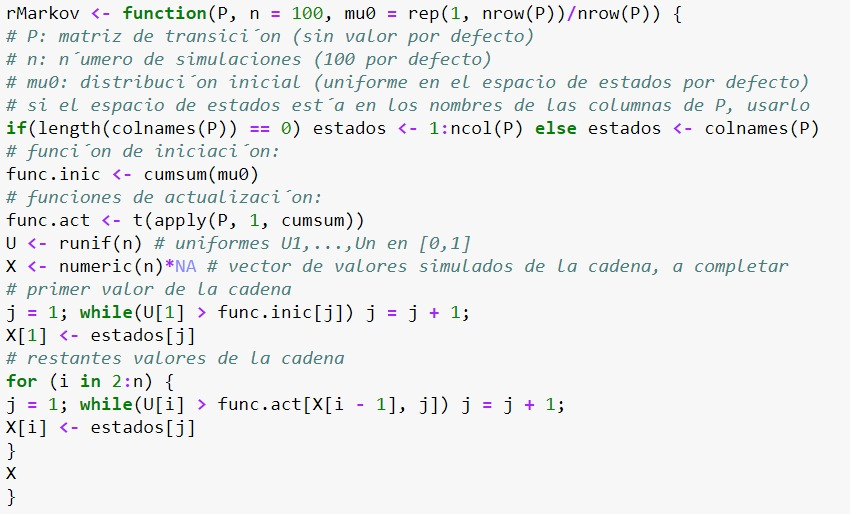
\includegraphics[scale=0.30]{fun1.jpeg}
	\captionof{figure}{Función que simula una cada de Markov.}
	\label{figura1}
\end{Figure}

Si consideramos un espacio de estados $E=\{A,C,G,T\}$ (A=adenina,C=citosina,G=guanina,T=timina)

\begin{Figure}
	\centering
	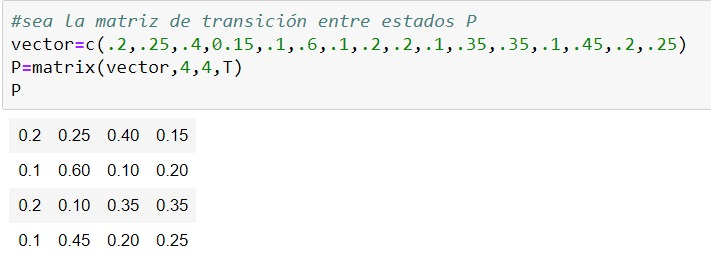
\includegraphics[scale=0.26]{fun2.jpeg}
	\captionof{figure}{Matriz de transición de la cadena de Markov.}
	\label{figura2}
\end{Figure}

\begin{Figure}
	\centering
	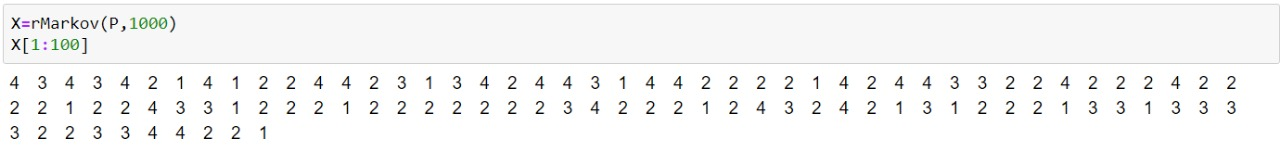
\includegraphics[scale=0.20]{fun3.jpeg}
	\captionof{figure}{Probando la función \textit{rMarkov}.}
	\label{figura3}
\end{Figure}

\begin{Figure}
	\centering
	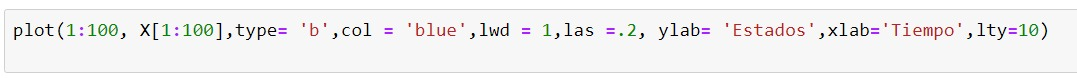
\includegraphics[scale=0.25]{fun4.jpeg}
	\captionof{figure}{Graficando la cadena de Markov.}
	\label{figura4}
\end{Figure}

\begin{Figure}
	\centering
	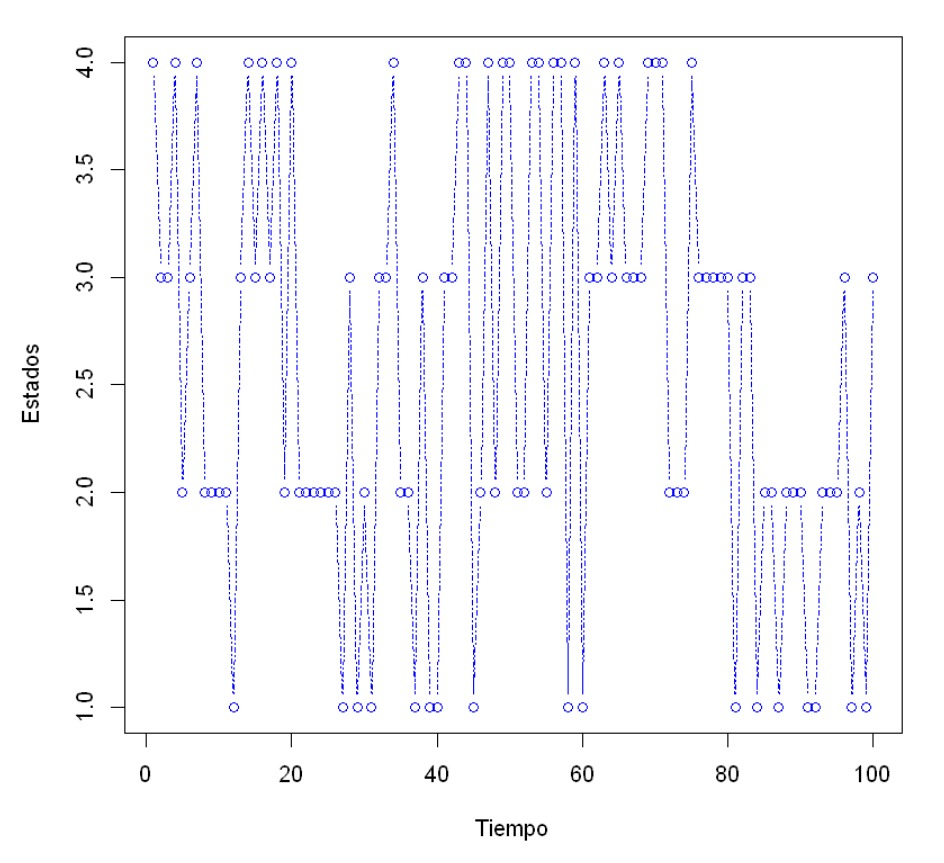
\includegraphics[scale=0.2]{fun5.jpeg}
	\captionof{figure}{Grafica Tiempo VS Estados.}
	\label{figura5}
\end{Figure}

\end{multicols}
\begin{thebibliography}{99}

\bibitem{Cd94} Autor, \emph{Ttulo}, Revista/Editor, (ao)

\end{thebibliography}
\end{document}